%%%%%%%%%%%%%%%%%%%%%%%%%%%%%%%%%%%%%%%%%%%%%%%%%%%%%%
\documentclass[11pt]{article}
%%%%%%%%%%%%%%%%%%%%%%%%%%%%%%%%%%%%%%%%%%%%%%%%%%%%%%

\usepackage{amsmath}
\usepackage{amsthm}
\usepackage{amssymb}
\usepackage{latexsym}
\usepackage{graphicx}
\usepackage{color}
\usepackage{verbatim}
\usepackage{float}
\usepackage{multicol}
\usepackage{xcolor}
\usepackage{listings}
\usepackage{tikz}
\usetikzlibrary{arrows.meta, positioning, calc}
\usetikzlibrary{decorations.pathmorphing}
\usepackage{tcolorbox}
\tcbuselibrary{breakable}

\newtcolorbox{solutionbox}{
  breakable,
  colback=blue!5!white,
  colframe=blue!50!black,
  title=Solution,
  sharp corners,
  boxrule=0.8pt
}

\newtcolorbox{hintbox}{
  breakable,
  colback=gray!10!white,
  colframe=gray!50!black,
  title=Hint,
  sharp corners,
  boxrule=0.5pt
}

% Unnumbered theorem
\newtheorem*{thm*}{Theorem}


\lstdefinelanguage{R}{
      keywords={if,else,while,for,in,next,break,function,TRUE,FALSE,NULL,Inf,NA,NaN,switch,repeat,return,require,library},
      keywordstyle=\color{blue}\bfseries,
      identifierstyle=\color{black},
      comment=[l]{\#},
      commentstyle=\color{gray}\ttfamily,
      string=[b]{"},
      stringstyle=\color{red}\ttfamily,
      morecomment=[l]{//},
      morestring=[b]{'},
      sensitive=true,
      morekeywords={print,summary,plot,lm,glm,data,frame,read.csv,write.csv,factor,levels,names,colnames,rownames,
      head,tail,str,dim,length,class,typeof,mode,is.na,is.null,is.finite,is.infinite,is.nan,as.numeric,as.character,
      as.factor,as.Date,as.POSIXct,as.matrix,as.data.frame,rbind,cbind,merge,subset,aggregate,tapply,apply,lapply,sapply,
      mapply,vapply,replicate,seq,rep,c,list,matrix,array,data.frame,table,hist,boxplot,barplot,pie,curve,lines,points,text,
      abline,legend,par,mtext,title,xlab,ylab,xlim,ylim,main,sub,col,pch,cex,lty,lwd,type,bg,fg,args,options,warnings,errors,
      message,stop,warning,error,try,tryCatch,withCallingHandlers,on.exit,debug,browser,trace,recover,options,getOption,setOption},
    }


\setlength{\textheight}{9in}
\setlength{\textwidth}{6in}
\addtolength{\topmargin}{-2cm}
\addtolength{\oddsidemargin}{-1cm}
\parindent=0in


\def\classnum{3810}
\def\classtitle{Probability}
\def\classtitleshort{Probability}
\def\classsec{001}
\def\classterm{Fall 2025}
\def\instructor{Robert Rostermundt}
%\def\hmwknum{\#2}


%%%%%%%%%%%%%%%%%%%%%%%%%%%%%%%%%%%%%%%%%%%%%%%%%%%%%%%%%
%%%%%%%%%%%%%%%%%%%%%%%%%  Colors  %%%%%%%%%%%%%%%%%%%%%%
%%%%%%%%%%%%%%%%%%%%%%%%%%%%%%%%%%%%%%%%%%%%%%%%%%%%%%%%%

\definecolor{Green}{rgb}{0,.5,0}
%use for definitions
\definecolor{Red}{rgb}{.8,.2,0}
%use for emphasis
\definecolor{Yellow}{rgb}{.6,.6,.1}
%use for part titles
\definecolor{Cyan}{rgb}{.2,.6,.7}
%use for comments
\definecolor{Purple}{rgb}{.4,0,1}
%use for examples
\definecolor{deepred}{rgb}{.53,.29,.24}
%use for important points
\definecolor{Black}{rgb}{0,0,0}
%use for washout
\definecolor{Grey}{rgb}{.45,.45,.45}
% use for theorems
\newcommand{\tred}[1]{\textcolor{Red}{#1}}
\newcommand{\tgreen}[1]{\textcolor{Green}{#1}}
\newcommand{\tcyan}[1]{\textcolor{Cyan}{#1}}
\newcommand{\tyellow}[1]{\textcolor{Yellow}{#1}}
\newcommand{\tpurple}[1]{\textcolor{Purple}{#1}}
\newcommand{\tblack}[1]{\textcolor{Black}{#1}}
\newcommand{\tgrey}[1]{\textcolor{Grey}{#1}}
\newcommand{\tdeepred}[1]{\textcolor{deepred}{#1}}
\newcommand{\ttt}[1]{\texttt{#1}}

%%%%%%%%%%%%%%%%%%%%%%%%%%%%%%%%%%%%%%%%%%%%%%%%%%%%%%%%%
%%%%%%%%%%%%%%%%%%%%%%%%%  Theorem Environments  %%%%%%%%
%%%%%%%%%%%%%%%%%%%%%%%%%%%%%%%%%%%%%%%%%%%%%%%%%%%%%%%%%

\theoremstyle{plain}
\newtheorem{thm}{Theorem}
\newtheorem{axiom}{Axiom}
\newtheorem{cor}{Corollary}
\newtheorem{lemma}{Lemma}
\newtheorem{prop}{Proposition}
\newtheorem{ques}{Question}
\theoremstyle{definition}
\newtheorem{defn}{Definition}
\theoremstyle{remark}
\newtheorem{remark}{Remark}
\theoremstyle{definition}
\newtheorem{ex}{Example}
\numberwithin{equation}{section}
\newtheorem{prob}{Problem}
\numberwithin{equation}{section}


%%%%%%%%%%%%%%%%%%%%%%%%%%%%%%%%%%%%%%%%%%%%%%%%%%%%%%%%%
%%%%%%%%%%%%%%%%%%%%%%%%%  Math    %%%%%%%%%%%%%%%%%%%%%%
%%%%%%%%%%%%%%%%%%%%%%%%%%%%%%%%%%%%%%%%%%%%%%%%%%%%%%%%%


\newcommand{\abs}[1]{\left\lvert{#1}\right\rvert}
\newcommand{\card}[1]{\lvert{#1}\rvert}
\newcommand{\union}{\cup}
\newcommand{\Union}{\bigcup}
\newcommand{\inter}{\cap}
\newcommand{\Inter}{\bigcap}
%\newcommand{\hint}[1]{\medskip\newline\emph{Hint: #1}}
%\newcommand{\note}[1]{\medskip\newline\emph{Note: #1}}
\newcommand{\points}[1]{[#1 points]}
\newcommand{\totalpoints}[1]{[#1 points total]}
\newcommand{\ds}{\displaystyle}
\newcommand{\ben}{\begin{enumerate}}
\newcommand{\een}{\end{enumerate}}
\newcommand{\bi}{\begin{itemize}}
\newcommand{\ei}{\end{itemize}}
\newcommand{\beq}{\begin{eqnarray*}}
\newcommand{\eeq}{\end{eqnarray*}}
\newcommand{\bieq}{\begin{IEEEeqnarray}{rCl}}
\newcommand{\bieqx}{\begin{IEEEeqnarray}{+rCl+x*}}
\newcommand{\eieq}{\end{IEEEeqnarray}}
\newcommand{\nn}{\nonumber}
%\renewcommand{\i}{\item}
\newcommand{\bpm}{\begin{pmatrix}}
\newcommand{\epm}{\end{pmatrix}}
\newcommand{\sol}{\indent{\bf\emph{Solution:}}}
\newcommand{\ssol}{\indent{\\[2mm]\bf\emph{Solution:}}\;}
\newcommand{\hint}{\indent{\bf\emph{Hint}:}\;}
\newcommand{\note}{\indent{\bf\emph{Note}:}\;}
\newcommand{\vsk}{\vskip 2mm}
%%%%%%%%%%%%%%%%%%%%%%%%% Calculus %%%%%%%%%%%%%%%%%%%%%%%%%%%%
\newcommand{\dd}[2]{\ds\frac{d}{d{#1}}\left[{#2}\right]}
\newcommand{\der}[2]{\ds\frac{d{#1}}{d{#2}}}
\newcommand{\lmt}[3]{\ds\lim_{{#1}\to{#2}}{#3}}
\renewcommand{\iint}[2]{\ds\int{#1}\,d{#2}}
\newcommand{\dint}[4]{\ds\int^{#4}_{#3}{#1}\,d{#2}}
\renewcommand{\Delta}{\triangle}
%%%%%%%%%%%%%%%%%%%%%%%%% Number Sets %%%%%%%%%%%%%%%%%%%%%%%%%%
\newcommand{\N}{\mathbb{N}}
\newcommand{\Z}{\mathbb{Z}}
\newcommand{\Q}{\mathbb{Q}}
\newcommand{\R}{\mathbb{R}}
\newcommand{\C}{\mathbb{C}}
\newcommand{\F}{\mathcal{F}}
\renewcommand{\P}{\mathbb{P}}
\newcommand{\E}{\mathcal{E}}
\renewcommand{\o}{\omega}
\renewcommand{\O}{\Omega}
%%%%%%%%%%%%%%%%%%%%%%%%% Vectors %%%%%%%%%%%%%%%%%%%%%%%%%%%%%
\newcommand{\x}{\bar{x}}
\renewcommand{\v}{\bar{v}}
\newcommand{\y}{\bar{y}}
\newcommand{\z}{\bar{z}}
\newcommand{\w}{\bar{w}}
\renewcommand{\u}{\bar{u}}
\renewcommand{\b}{\bar{b}}
\newcommand{\e}{\bar{e}}
\renewcommand{\a}{\vec{a}}
\renewcommand{\r}{\vec{r}}
\newcommand{\vv}{\vec{v}}
\newcommand{\vecPQ}[2]{\overrightarrow{#1}{#2}}
\newcommand{\vecV}[1]{\overrightarrow{#1}}
\newcommand{\la}{\langle}
\newcommand{\ra}{\rangle}
%%%%%%%%%%%%%%%%%%%%%%%%%%% Vector Spaces %%%%%%%%%%%%%%%%%%%%
\newcommand{\rn}{\ensuremath{\mathbb{R}^n}}
\renewcommand{\rm}{\ensuremath{\mathbb{R}^m}}
\newcommand{\re}{\mathbb{R}}
\newcommand{\Pn}{\mathbb{P}_n}
\newcommand{\B}{\mathcal{B}}
%%%%%%%%%%%%%%%%%%%%%%%%%%% Graphics %%%%%%%%%%%%%%%%%%%%%%%%
\newcommand{\cg}[2]{\begin{center}
\includegraphics[scale={#1}]{{#2}}
\end{center}}
\makeatletter
\def\imod#1{\allowbreak\mkern10mu({\operator@font mod}\,\,#1)}
\makeatother

%%%%%%%%%%%%%%%%%%%%%%%%%%%%%%%%%%%%%%%%%%%%%%%%%%%%%%%%%%%%%%%%%%%%%%%%%%%%%%%%%%%%%%%%%%%%%%
%%%%%%%%%%%%%%%%%%%%%%%%%%%%%% Defined Fonts %%%%%%%%%%%%%%%%%%%%%%%%%%%%%%%%%%%%%%%%%%%%%%%%%
%%%%%%%%%%%%%%%%%%%%%%%%%%%%%%%%%%%%%%%%%%%%%%%%%%%%%%%%%%%%%%%%%%%%%%%%%%%%%%%%%%%%%%%%%%%%%%

\font\minihelv=phvr at 6pt
\font\helv=phvr at 10pt
\font\medhelv=phvr at 16pt
\font\bighelv=phvr at 20pt
\font\hugehelv=phvr at 36pt
\font\mybigfont=phvr at 16pt
\font\mymediumfont=phvr at 14pt
\font\mediumhelv=phvr at 14pt
\font\mybfit=ptmbi at 12pt


%%%%%%%%%%%%%%%%%%%%%%%%%%%%%%%%%%%%%%%%%%%%%%%%%%%%%%%%%%%%%%%%%%%%%%%%%%%%%%%%%%%%%%%%%%%%%%%
%%%%%%%%%%%%%%%%%%%%%%%%%%%%%% Other Commands %%%%%%%%%%%%%%%%%%%%%%%%%%%%%%%%%%%%%%%%%%%%%%%%%
%%%%%%%%%%%%%%%%%%%%%%%%%%%%%%%%%%%%%%%%%%%%%%%%%%%%%%%%%%%%%%%%%%%%%%%%%%%%%%%%%%%%%%%%%%%%%%%
%\setlength\fboxrule{.5pt}
%\newcommand{\latexpicborder}[3]{
%\setlength\fboxsep{30pt}
%\begin{figure}[hb]
%\begin{center}
%\fbox{
%\input{#1}
%}
%\caption{#2}
%\label{#3}
%\end{center}
%\end{figure}
%\setlength\fboxsep{0pt}
%}
%
%\newcommand{\latexpic}[2]{
%\begin{figure}[hb]
%\begin{center}
%\input{#1}
%\vspace*{8mm}
%\caption{#2}
%\end{center}
%\end{figure}
%}

%\begin{minipage}[b]{0.6\linewidth}
%......
%\end{minipage}
%\hspace{0.5cm}
%\begin{minipage}[t]{0.4\linewidth}
%\centering
%\includegraphics[scale=.5]{m1401_ex3_g4.eps}
%\end{minipage}
%\end{figure}


%%%%%%%%%%%%%%%%%%%%%%%%%%%%%%%%%%%%%%%%%%%%%%%%%%%%%%%%%%%%%%%%%%%%%%%%%%%%%%%%%%%%%%%%%%%%%%
%%%%%%%%%%%%%%%%%%%%%%%%%%% IEEEeqnarray Notes %%%%%%%%%%%%%%%%%%%%%%%%%%%%%%%%%%%%%%%%%%%%%%%
%%%%%%%%%%%%%%%%%%%%%%%%%%%%%%%%%%%%%%%%%%%%%%%%%%%%%%%%%%%%%%%%%%%%%%%%%%%%%%%%%%%%%%%%%%%%%%


%Any number of columns can be specified with IEEEeqnarray: {c} will give only one
%column with all entries centered, or {rCll} would add a fourth, left-justified
%column to use for comments. Moreover, beside l, c, r, L, C, R for math mode
%entries there are also s, t, u for left, centered, and right text mode entries.
%Additional space can be added with . and / and ? in increasing order.
%
%
%\begin{proof}
%This is a proof that ends
%with an equation array:
%\begin{IEEEeqnarray*}{+rCl+x*}
%a & = & b + c \\
%& = & d + e. & \qedhere
%\end{IEEEeqnarray*}
%\end{proof}
%Note that the + in {+rCl+x*} denotes stretchable spaces, one on the left
%of the equations (which, if not specified, will be done automatically by
%IEEEeqnarray!) and one on the right of the equations. But now on the right,
%after the stretching column, we add an empty column x. This column will be
%only needed on the last line when we will put the \qedhere command there.
%Finally, we specify a *. This is a null-space that prevents IEEEeqnarray to
%add another unwanted +-space!


% The following environments enable custom numbering of theorems so that the numbers agree % with the numbering in the textbook being used. 
%
%  Usage examples:
%\begin{customthm}{2.2}\label{eight}
%Every theorem must be numbered by hand.
%\end{customthm}
%
%Here is a reference to theorem~\ref{eight}.
%
%\begin{customthm}{2.3}[Parenthetical comment]\label{nine}
%Statement
%\end{customthm}
%
%Here is a reference to theorem~\ref{nine}


\newtheorem{innercustomthm}{Theorem}
\newenvironment{customthm}[1]
  {\renewcommand\theinnercustomthm{#1}\innercustomthm}
  {\endinnercustomthm}
  
  \newtheorem{innercustomprop}{Proposition}
\newenvironment{customprop}[1]
  {\renewcommand\theinnercustomprop{#1}\innercustomprop}
  {\endinnercustomprop}
  
    \newtheorem{innercustomlem}{Lemma}
\newenvironment{customlem}[1]
  {\renewcommand\theinnercustomlem{#1}\innercustomlem}
  {\endinnercustomlem}
  
    \newtheorem{innercustomconj}{Conjecture}
\newenvironment{customconj}[1]
  {\renewcommand\theinnercustomconj{#1}\innercustomconj}
  {\endinnercustomconj}
  
    \newtheorem{innercustomclaim}{Claim}
\newenvironment{customclaim}[1]
  {\renewcommand\theinnercustomclaim{#1}\innercustomclaim}
  {\endinnercustomclaim}
  
    \newtheorem{innercustomcor}{Corollary}
\newenvironment{customcor}[1]
  {\renewcommand\theinnercustomcor{#1}\innercustomcor}
  {\endinnercustomcor}
  
    \newtheorem{innercustomdef}{Definition}
\newenvironment{customdef}[1]
  {\renewcommand\theinnercustomdef{#1}\innercustomdef}
  {\endinnercustomdef}
  
    \newtheorem{innercustomex}{Example}
\newenvironment{customex}[1]
  {\renewcommand\theinnercustomex{#1}\innercustomex}
  {\endinnercustomex}
  
    \newtheorem{innercustomass}{Assumption}
\newenvironment{customass}[1]
  {\renewcommand\theinnercustomass{#1}\innercustomass}
  {\endinnercustomass}
  
      \newtheorem{innercustomax}{Axiom}
\newenvironment{customax}[1]
  {\renewcommand\theinnercustomax{#1}\innercustomax}
  {\endinnercustomax}
  

\vfuzz2pt % Don't report over-full v-boxes if over-edge is small
\hfuzz2pt % Don't report over-full h-boxes if over-edge is small

\renewcommand{\ni}{\noindent}


%%%%%%%%%%%%%%%%%%%%%%%%%%%%%%%%%%%%%%%%%%%%%%%%%%%%%%
%%%%%%%%%%%%%%%%%%%%%%%%%%%%%%%%%%%%%%%%%%%%%%%%%%%%%%

\pagestyle{myheadings}

%%%%%%%%%%%%%%%%%%%%%%%%%%%%%%%%%%%%%%%%%%%%%%%%%%%%%%

%%%%%%%%%%%%%%%%%%%%%%%%%%%%%%%%%%%%%%%%%%%%%%%%%%%%%%
%%%%%%%%%%%%%%%%%%%%%%%%%   Document Body   %%%%%%%%%%
%%%%%%%%%%%%%%%%%%%%%%%%%%%%%%%%%%%%%%%%%%%%%%%%%%%%%%

%\def\classnum{3810}
%\def\classtitle{Probability}
%\def\classtitleshort{Probability}
%\def\classsec{001}
%\def\classterm{Fall 2025}
%\def\instructor{Robert Rostermundt}
\def\printsol{0}


	\title{\vspace{-1in}Math\classnum\;-\;\classtitle\\
	Section\;\classsec\;-\;\classterm\\
	Notes: Joint Probability Distributions}
	\author{University of Colorado Denver / College of Liberal Arts 	and Sciences}
	\date{Department of Mathematics - \instructor}

	\markright{Math\classnum\;-\;\classtitleshort, UCD, \classterm, \instructor}



%%%%%%%%%%%%%%%%%%%%%%%%%%%%%%%%%%%%%%%%%%%%%%%%%%%%%%
\begin{document}\maketitle\thispagestyle{empty}
%%%%%%%%%%%%%%%%%%%%%%%%%%%%%%%%%%%%%%%%%%%%%%%%%%%%%%


%%%%%%%%%%%%%%%%%%%%%%%%%%%%%%%%%%%%%%%%%%%%%%%%%%%%%%%%%%%%%%%%%%%%%%%%%%%%%%%%%%%%%%%%%%%%%%%%%%%%%%
\vspace*{2mm}
\hrule
\vskip 8mm

%%%%%%%%%%%%%%%%%%%%%%%%%%%%%%%%%%%%%%%%%%%%%%%%%%%%%%%%%%%%%%%%%%%%%%%%%
%%%%%%%%%%%%%%%%%%%%%%%%%%%%%%%%%%%%%%%%%%%%%%%%%%%%%%%%%%%%%%%%%%%%%%%%%

%%%%%%%%%%%%%%%%%%%%%%%%%%%%%%%%%%%%%%%%%%%%%%%%%%%%%%%%%%%%%%%%%%%%%%%%%%%%%%%%%%%%%%%%%%%%%%%%%%%%%%
\section*{Motivation: Joint Distributions}
%%%%%%%%%%%%%%%%%%%%%%%%%%%%%%%%%%%%%%%%%%%%%%%%%%%%%%%%%%%%%%%%%%%%%%%%%%%%%%%%%%%%%%%%%%%%%%%%%%%%%%

Many experiments naturally produce more than one numerical outcome.
When we record these outcomes together, we obtain a \emph{pair} of random quantities
rather than a single one.

\medskip

\textbf{Example: Rolling two dice.}
When two fair dice are rolled, the outcome can be represented as an ordered pair
\[(X,Y) = (\text{first die}, \text{second die}).\]
Rather than studying $X$ or $Y$ alone, we may want to answer questions such as:
\begin{itemize}
\item What is the probability that both dice show the same value?
\item What is the probability that the sum exceeds $9$?
\item Are the values of the two dice independent?
\end{itemize}

To answer these questions, we need a way to assign probabilities to \emph{pairs} of values.
This leads to the idea of a \emph{joint probability distribution}.

%%%%%%%%%%%%%%%%%%%%%%%%%%%%%%%%%%%%%%%%%%%%%%%%%%%%%%%%%%%%%%%%%%%%%%%%%%%%%%%%%%%%%%%%%%%%%%%%%%%%%%
\section*{Joint Random Variables:}
%%%%%%%%%%%%%%%%%%%%%%%%%%%%%%%%%%%%%%%%%%%%%%%%%%%%%%%%%%%%%%%%%%%%%%%%%%%%%%%%%%%%%%%%%%%%%%%%%%%%%%

\begin{defn}
Let $X$ and $Y$ be random variables defined on the same experiment.
The ordered pair
\[(X,Y)\]
is called a \textbf{\emph{joint random variable}}.
\end{defn}

\ni Each outcome of the experiment produces a numerical pair $(X,Y)\in\mathbb R^2$.
Probabilities are then assigned to events of the form
\[(X,Y)\in A,\]
where $A$ is a subset of the plane.

%%%%%%%%%%%%%%%%%%%%%%%%%%%%%%%%%%%%%%%%%%%%%%%%%%%%%%%%%%%%%%%%%%%%%%%%%%%%%%%%%%%%%%%%%%%%%%%%%%%%%%
\section*{Discrete Joint Distributions:}
%%%%%%%%%%%%%%%%%%%%%%%%%%%%%%%%%%%%%%%%%%%%%%%%%%%%%%%%%%%%%%%%%%%%%%%%%%%%%%%%%%%%%%%%%%%%%%%%%%%%%%

\begin{defn}
A joint random variable $(X,Y)$ is called \textbf{\emph{discrete}} if it takes values
in a finite or countable set of ordered pairs.
The function
\[p_{_{X,Y}}(x,y)=\P(X=x,\;Y=y)
\]
is called the \textbf{\emph{joint probability mass function (pmf)}}.
\end{defn}

\ni The joint pmf satisfies
\[p_{_{X,Y}}(x,y)\ge 0,\qquad\sum_x\sum_y p_{_{X,Y}}(x,y)=1.\]

\ni Probabilities are computed by summing over the relevant pairs:
\[\P\big((X,Y)\in A\big)=\sum_{(x,y)\in A} p_{_{X,Y}}(x,y).\]

\ni Joint pmfs are often displayed in table form, which makes many probabilities
easy to compute directly.

%%%%%%%%%%%%%%%%%%%%%%%%%%%%%%%%%%%%%%%%%%%%%%%%%%%%%%%%%%%%%%%%%%%%%%%%%%%%%%%%%%%%%%%%%%%%%%%%%%%%%%
\section*{Continuous Joint Distributions:}
%%%%%%%%%%%%%%%%%%%%%%%%%%%%%%%%%%%%%%%%%%%%%%%%%%%%%%%%%%%%%%%%%%%%%%%%%%%%%%%%%%%%%%%%%%%%%%%%%%%%%%

\begin{defn}
A joint random variable $(X,Y)$ is called \textbf{\emph{continuous}} if there exists a
nonnegative function $f_{X,Y}:\mathbb R^2\to[0,\infty)$ such that
\[\P\big((X,Y)\in A\big)=\int_A f_{_{X,Y}}(x,y)\,dx\,dy\]
for all regions $A\subseteq\mathbb R^2$.
The function $f_{_{X,Y}}$ is called the \textbf{\emph{joint probability density function (pdf)}}.
\end{defn}

\ni In this setting, probabilities are interpreted geometrically:
they correspond to the volume under the surface $z=f_{_{X,Y}}(x,y)$ above the region $A$.



%%%%%%%%%%%%%%%%%%%%%%%%%%%%%%%%%%%%%%%%%%%%%%%%%%%%%%%%%%%%%%%%%%%%%%%%%%%%%%%%%%%%%%%%%%%%%%%%%%%%%%
\section*{From Joint Mass/Density to the Joint Distribution (and Back)}
%%%%%%%%%%%%%%%%%%%%%%%%%%%%%%%%%%%%%%%%%%%%%%%%%%%%%%%%%%%%%%%%%%%%%%%%%%%%%%%%%%%%%%%%%%%%%%%%%%%%%%

For a pair of random variables $(X,Y)$, there are two closely related objects:
\begin{itemize}
\item the \textbf{joint distribution function}
\[F_{_{X,Y}}(x,y)=\P(X\le x,\;Y\le y),\]
\item and the \textbf{joint probability mass function} or \textbf{joint density function}.
\end{itemize}

This section shows how to move between these objects using summation,
integration, and differentiation.

%%%%%%%%%%%%%%%%%%%%%%%%%%%%%%%%%%%%%%%%%%%%%%%%%%%%%%%%%%%%%%%%%%%%%%%%%%%%%%%%%%%%%%%%%%%%%%%%%%%%%%
\subsection*{Discrete Case}
%%%%%%%%%%%%%%%%%%%%%%%%%%%%%%%%%%%%%%%%%%%%%%%%%%%%%%%%%%%%%%%%%%%%%%%%%%%%%%%%%%%%%%%%%%%%%%%%%%%%%%

Suppose $(X,Y)$ is discrete with joint pmf $p_{_{X,Y}}(x,y)$.

\medskip

\ni The joint distribution function is obtained by summing the joint pmf over
all points in the lower-left quadrant:
\[F_{_{X,Y}}(x,y)=\sum_{x_i\le x}\sum_{y_j\le y} p_{_{X,Y}}(x_i,y_j).
\]

\ni Thus, $F_{_{X,Y}}(x,y)$ accumulates the probabilities of all outcomes
for which $X\le x$ and $Y\le y$.

\medskip

\textbf{Recovering the pmf:} Because $F_{_{X,Y}}$ jumps at each point $(x,y)$, the joint pmf can be recovered
using finite differences:
\[p_{_{X,Y}}(x,y)=F_{_{X,Y}}(x,y)-F_{_{X,Y}}(x^-,y)-F_{_{X,Y}}(x,y^-)+F_{_{X,Y}}(x^-,y^-),\]
where $x^-$ and $y^-$ denote values just smaller than $x$ and $y$.

\medskip

\textbf{Example.}
For two fair dice,
\[F_{_{X,Y}}(x,y)=\frac{1}{36}\,\#\{(i,j): i\le x,\; j\le y\},\]
and the pmf $p_{_{X,Y}}(x,y)=1/36$ is recovered by taking differences across the jumps of $F_{_{X,Y}}$.

%%%%%%%%%%%%%%%%%%%%%%%%%%%%%%%%%%%%%%%%%%%%%%%%%%%%%%%%%%%%%%%%%%%%%%%%%%%%%%%%%%%%%%%%%%%%%%%%%%%%%%
\subsection*{Continuous Case}
%%%%%%%%%%%%%%%%%%%%%%%%%%%%%%%%%%%%%%%%%%%%%%%%%%%%%%%%%%%%%%%%%%%%%%%%%%%%%%%%%%%%%%%%%%%%%%%%%%%%%%

Suppose $(X,Y)$ is continuous with joint pdf $f_{_{X,Y}}(x,y)$.

\medskip

\ni The joint distribution function is obtained by integrating the joint density
over the rectangle $(-\infty,x]\times(-\infty,y]$:
\[F_{_{X,Y}}(x,y)=\int^{u=x}_{-\infty}\int^{v=y}_{-\infty}f_{_{X,Y}}(u,v)\,dv\,du.\]

\ni This integral accumulates probability over all outcomes with
$X\le x$ and $Y\le y$.

\medskip

\textbf{Recovering the density.}
If $F_{_{X,Y}}$ is differentiable, the joint density is obtained by taking partial derivatives:
\[f_{_{X,Y}}(x,y)=\frac{\partial^2}{\partial x\,\partial y} F_{_{X,Y}}(x,y).\]

\medskip

\textbf{Example.}
Suppose
\[f_{_{X,Y}}(x,y)=\left\{\begin{array}{lcl}
2&:& 0\le y\le x\le 1,\\
0&:& \text{Otherwise}.
\end{array}
\right.\]

Then
\[F_{_{X,Y}}(x,y)=\int^{u=\min(x,1)}_{u=0}\int^{v=\min(y,u)}_{v=0} 2\,dv\,du,\]
and differentiating $F_{_{X,Y}}(x,y)$ with respect to $x$ and $y$
recovers the joint density $f_{_{X,Y}}(x,y)$.

%%%%%%%%%%%%%%%%%%%%%%%%%%%%%%%%%%%%%%%%%%%%%%%%%%%%%%%%%%%%%%%%%%%%%%%%%%%%%%%%%%%%%%%%%%%%%%%%%%%%%%
\subsection*{Summary}
%%%%%%%%%%%%%%%%%%%%%%%%%%%%%%%%%%%%%%%%%%%%%%%%%%%%%%%%%%%%%%%%%%%%%%%%%%%%%%%%%%%%%%%%%%%%%%%%%%%%%%

\begin{center}
\begin{tabular}{c c c}
\textbf{Object} & \textbf{Operation} & \textbf{Result} \\ \hline
Joint pmf & summation & joint distribution \\
Joint pdf & double integration & joint distribution \\
Joint distribution & finite differences & joint pmf \\
Joint distribution & partial derivatives & joint pdf
\end{tabular}
\end{center}



%%%%%%%%%%%%%%%%%%%%%%%%%%%%%%%%%%%%%%%%%%%%%%%%%%%%%%%%%%%%%%%%%%%%%%%%%%%%%%%%%%%%%%%%%%%%%%%%%%%%%%
\section*{Worked Example: A Joint Density with Triangular Support}
%%%%%%%%%%%%%%%%%%%%%%%%%%%%%%%%%%%%%%%%%%%%%%%%%%%%%%%%%%%%%%%%%%%%%%%%%%%%%%%%%%%%%%%%%%%%%%%%%%%%%%

Let $(X,Y)$ have joint density
\[f_{_{X,Y}}(x,y)=\left\{\begin{array}{ccl}
24x(1-x-y)&:& x\ge 0,\; y\ge 0,\; x+y\le 1,\\[2mm]
0&:& \text{Otherwise}.
\end{array}
\right.\]

The support is a triangular (wedge-shaped) region in the first quadrant.

\begin{figure}[h!]
\centering
\includegraphics[scale=0.9]{joint_density_plot.jpg}
\caption{Plot of Joint Density Function $f_{_{X,Y}}(x,y)$.}
\label{fig:jointdensity}
\end{figure}


%%%%%%%%%%%%%%%%%%%%%%%%%%%%%%%%%%%%%%%%%%%%%%%%%%%%%%%%%%%%%%%%%%%%%%%%%%%%%%%%%%%%%%%%%%%%%%%%%%%%%%
\subsection*{Problem 1: Verify that $f_{_{X,Y}}$ Is a Valid Joint Density}
%%%%%%%%%%%%%%%%%%%%%%%%%%%%%%%%%%%%%%%%%%%%%%%%%%%%%%%%%%%%%%%%%%%%%%%%%%%%%%%%%%%%%%%%%%%%%%%%%%%%%%

We must check that $f_{X,Y}(x,y)\ge 0$ on its support and that
\[\int^{x=1}_{x=0}\ds\int^{y=1-x}_{y=0}24x(1-x-y)\,dy\,dx = 1.\]
Compute the inner integral:
\[\int^{y=1-x}_{y=0}24x(1-x-y)\,dy=24x\left[(1-x)y-\frac{y^2}{2}\right]^{y=1-x}_{y=0}=24x\frac{(1-x)^2}{2}.\]
Now integrate with respect to $x$:
\[\int^{x=1}_{x=0}12x(1-x)^2\,dx=12\int^{x=1}_{x=0}x-2x^2+x^3\,dx=12\left(\frac{1}{2}-\frac23+\frac{1}{4}\right)=1.\]

So $f_{_{X,Y}}$ is a valid joint density. Here is a diagram of the support of the joint distribution.

\begin{figure}[h!]
	\centering
		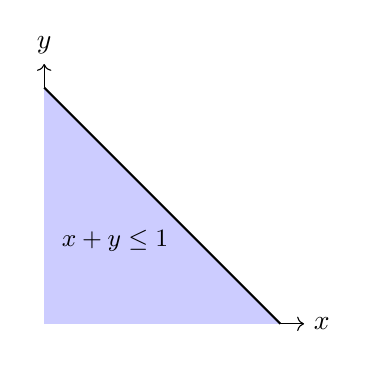
\begin{tikzpicture}[scale=3]
\draw[->] (0,0)--(1.1,0) node[right] {$x$};
\draw[->] (0,0)--(0,1.1) node[above] {$y$};
\fill[blue!20] (0,0)--(1,0)--(0,1)--cycle;
\draw[thick] (1,0)--(0,1);
\node at (0.3,0.35) {\small $x+y\le 1$};
		\end{tikzpicture}
\caption{Support of $f_{_{X,Y}}(x,y)=24x(1-x-y)$.}
\end{figure}


%--------------------------------------------
% Calculate the joint distribution
%--------------------------------------------


\vfill\eject

%%%%%%%%%%%%%%%%%%%%%%%%%%%%%%%%%%%%%%%%%%%%%%%%%%%%%%%%%%%%%%%%%%%%%%%%%%%%%%%%%%%%%%%%%%%%%%%%%%%%%%
\subsection*{Problem 2: Compute the Joint Distribution Function}
%%%%%%%%%%%%%%%%%%%%%%%%%%%%%%%%%%%%%%%%%%%%%%%%%%%%%%%%%%%%%%%%%%%%%%%%%%%%%%%%%%%%%%%%%%%%%%%%%%%%%%

We next compute the joint distribution function $F_{_{X,Y}}(x,y)$. Recall that
\vskip 2mm
\[F_{_{X,Y}}(x,y)=\P\big(X\le x,\,Y\le y\big)=\ds\int^{u=x}_{-\infty}\ds\int^{v=y}_{-\infty}f_{_{X,Y}}(u,v)\,dvdu.\]
Because the support is a triangular region, the distribution function will have a piece-wise description and there are a number of different integrals that must be computed, depending on the location of the point $(x,y)$. See regions $A,B,C,D$, and $E$ in Figure~\ref{fig:jointdistregions}.

\begin{figure}[h!]
	\centering
		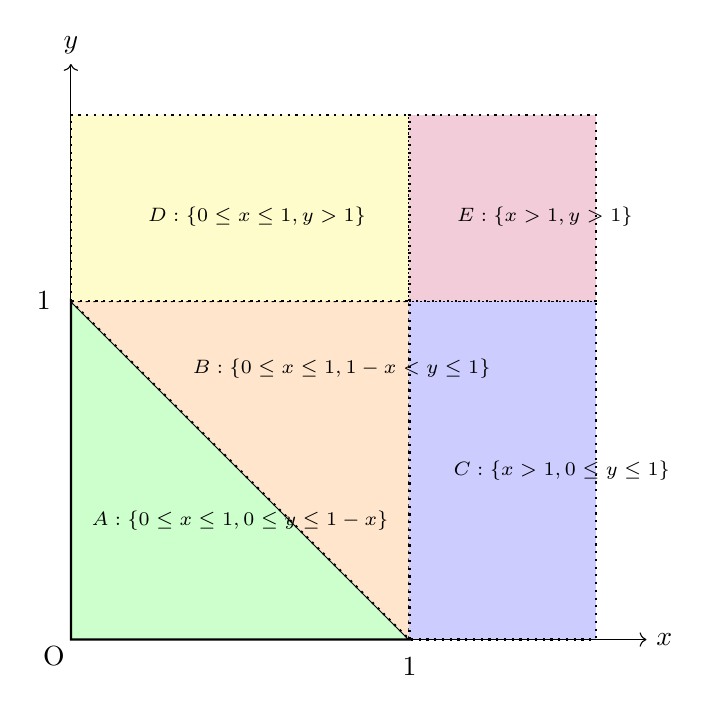
\begin{tikzpicture}[scale=4.3]
% Region A: 0<=x<=1, 0<=y<=1-x
\fill[green!20] (0,0) -- (1,0) -- (0,1) -- cycle;
\draw[thick] (0,0) -- (1,0) -- (0,1) -- cycle;
% Region B: 0<=x<=1, 1-x<y<=1
\fill[orange!20] (0,1) -- (1,0) -- (1,1) -- (0,1) -- cycle;
\draw[thick,dotted] (0,1) -- (1,0) -- (1,1) -- (0,1) -- cycle;
% Region C: x>1, 0<=y<=1
\fill[blue!20] (1,0) rectangle (1.55,1);
\draw[thick,dotted] (1,0) rectangle (1.55,1);
% Region D: 0<=x<=1, y>1
\fill[yellow!20] (0,1) rectangle (1,1.55);
\draw[thick,dotted] (0,1) rectangle (1,1.55);
% Region E: x>1, y>1
\fill[purple!20] (1,1) rectangle (1.55,1.55);
\draw[thick,dotted] (1,1) rectangle (1.55,1.55);
% Region Labels
\node at (0.5,0.35) {\scriptsize $A: \{0\le x\le1, 0\le y\le 1-x\}$};
\node at (0.8,0.8) {\scriptsize $B: \{0\le x\le1, 1-x<y\le1\}$};
\node at (1.45,0.5) {\scriptsize $C: \{x>1, 0\le y\le1\}$};
\node at (0.55,1.25) {\scriptsize $D: \{0\le x\le1, y>1\}$};
\node at (1.4,1.25) {\scriptsize $E: \{x>1, y>1\}$};
\node at (1,-0.08) {$1$};
\node at (-0.08,1) {$1$};
% Axes
\draw[->] (0,0) -- (1.7,0) node[right] {$x$};
\draw[->] (0,0) -- (0,1.7) node[above] {$y$};
% Origin
\node at (-0.05,-0.05) {O};
		\end{tikzpicture}
\caption{Regions where joint distribution $F_{X,Y}(x,y)$ is non-zero.}
\label{fig:jointdistregions}
\end{figure}
\vskip 5mm
After our calculations we will find that
\vskip 5mm
\[F_{_{X,Y}}(x,y)=\left\{\begin{array}{lcl}
0&:& x<0 \text{ or } y<0 \\[3mm]
12 x^2 y - 8 x^3 y - 6 x^2 y^2 &:& 0 \le x \le 1,\, 0 \le y \le 1-x \\[3mm]
6 x^2 - 8 x^3 + 3 x^4 + 4 y^3+\cdots && \\[1mm]
- 3 y^4 + 2 y (2 - 3 y + y^3)-1 &:& x+y>1,\,0<x,y<1\\[3mm]
4 y - 6 y^2 + 4 y^3 - y^4 &:& x>1,\, 0 \le y \le 1 \\[3mm]
6 x^2 - 8 x^3 + 3 x^4 &:& y>1,\,0 \le x \le 1 \\[3mm]
1 &:& x\ge 1,\, y \ge 1
\end{array}
\right.\]

\vfill\eject

{\bf\emph{CDF Calculations for }}$f_{X,Y}(x,y)=24x(1-x-y)$:
\vskip 5mm
The joint density has support 
\[R_{_{X,Y}}=\{(x,y)\mid x\ge 0, y\ge 0, x+y \le 1\}.\]
We will provide calculations for three cases: Region A - $0 < x < 1$, $0 < y \le 1-x$ (inside the triangle); Region B - $0 < x < 1$, $1-x < y < 1$ (above the triangle); and Region C. 
\vskip 5mm
{\bf\emph{Region A:}} $0 < x < 1$, and $0 < y \le 1-x$ (Inside the Triangle)
\vskip 5mm
By definition of the CDF:
\[F_{_{X,Y}}(x,y)=\P(X\le x,Y\le y)=\ds\int^{u=x}_{u=0}\ds\int^{v=y}_{v=0}f_{_{X,Y}}(u,v)\,dvdu\]
\vskip 2mm
\emph{Step 1: Inner integral over $v$}
\[\ds\int^{v=y}_{v=0}24u(1-u-v)\,dv=24u\int^{v=y}_{v=0}(1-u-v)\,dv=24u\Big[(1-u)v-\frac{v^2}{2}\Big]^{v=y}_{v=0}
=24u\left((1-u)y-\frac{y^2}{2}\right)\]
\vskip 2mm
\emph{Step 2: Outer integral over $u$}
\[\ds\int^{u=x}_{u=0}24u\left((1-u)y-\frac{y^2}{2}\right)\,du=\ds\int^{u=x}_{u=0}24u(1-u)y-12uy^2\,du\]
\vskip 2mm
Evaluating this integral with respect to $u$ gives us $F_{_{X,Y}}(x,y)=12x^2y-8x^3y-6x^2y^2$ when $0<x,y$ and $x+y<1$.
\vskip 5mm
---
\vskip 5mm

{\bf\emph{Region B:}} $x+y>1$, $0<x<1$, and $0<y<1$ (above the triangle)
\vskip 5mm
Here $(x,y)$ lies outside the triangular support (see Figure~\ref{fig:integrationregionB}) and we use two integrals. 
\[F_{_{X,Y}}(x,y)=\ds\int^{u=1-y}_{u=0}\ds\int^{v=y}_{v=0}24u(1-u-v)\,dvdu+\ds\int^{u=x}_{u=1-y}\ds\int^{v=1-u}_{v=0}24u(1-u-v)\,dvdu\]

We leave the computations to the reader and find when $x+y>1$, $0<x<1$, and $0<y<1$ we have
\[F_{_{X,Y}}(x,y)=6x^2-8x^3+3x^4+4y^3-3y^4+2y(2-3y+y^3)-1.\]


\begin{figure}[h!]
	\centering
		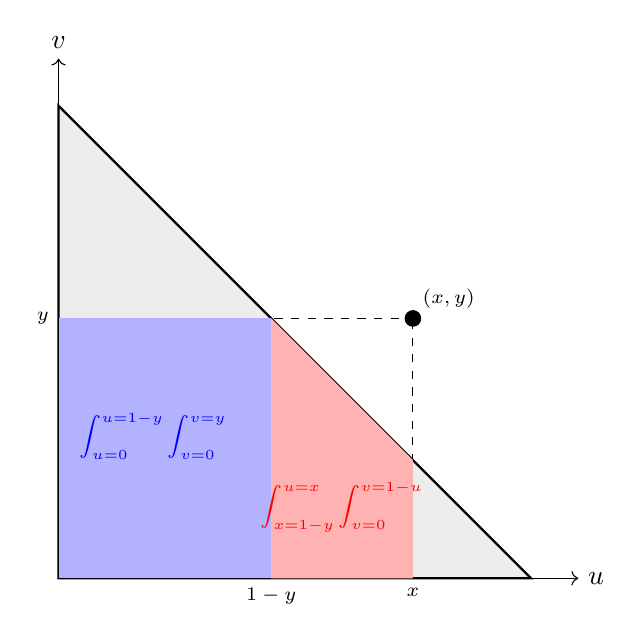
\begin{tikzpicture}[scale=6]
% Axes
\draw[->] (0,0) -- (1.1,0) node[right] {$u$};
\draw[->] (0,0) -- (0,1.1) node[above] {$v$};
% Support triangle
\fill[gray!15] (0,0) -- (1,0) -- (0,1) -- cycle;
\draw[thick] (0,0) -- (1,0) -- (0,1) -- cycle;
\node at (0.35,0.35) {\scriptsize $u+v\le1$};
% Parameters (example point)
\coordinate (X) at (0.75,0.55); % x+y>1
% Horizontal line v = y
\draw[dashed] (0,0.55) -- (0.75,0.55);
\node[left] at (0,0.55) {\scriptsize $y$};
% Vertical lines u = 1-y and u = x
\draw[dashed] (0.45,0) -- (0.45,0.55);
\node[below] at (0.45,0) {\scriptsize $1-y$};
\draw[dashed] (0.75,0) -- (0.75,0.55);
\node[below] at (0.75,0) {\scriptsize $x$};
% First integration region (blue)
\fill[blue!30]
(0,0) -- (0.45,0) -- (0.45,0.55) -- (0,0.55) -- cycle;
\node[blue] at (0.2,0.3)
{\scriptsize $\ds\int^{u=1-y}_{u=0}\ds\int^{v=y}_{v=0}$};
% Second integration region (correct trapezoid)
\fill[red!30]
(0.45,0) --
(0.75,0) --
(0.75,0.25) --
(0.45,0.55) -- cycle;
\node[red] at (0.6,0.15)
{\scriptsize $\ds\int^{u=x}_{x=1-y}\ds\int^{v=1-u}_{v=0}$};
% Point (x,y)
\fill (0.75,0.55) circle (0.5pt);
\node[above right] at (0.75,0.55) {\scriptsize $(x,y)$};
		\end{tikzpicture}
\caption{Integration when $(x,y)$ in Region B.}
\label{fig:integrationregionB}
\end{figure}

\vskip 5mm
---
\vskip 5mm

{\bf\emph{Region C:}} $x>1$, $0<y<1$
\vskip 5mm
We set up the iterated integral as
\[\int^{v=y}_{v=0}\int^{u=1-v}_{u=0}24u(1-u-v)\,dudv.\]
Evaluating this integral gives the distribution when $x>1$, $0<y<1$ as
\[F_{_{X,Y}}(x,y)=4y-6y^2+4y^3-y^4.\]
%\vskip 5mm
%\paragraph{Remark:} Notice that in this region the CDF no longer depends on $x$, because the support is capped by the line $x+y=1$.
\vskip 5mm
See Figure~\ref{fig:distributionplot} for a plot of the distribution function $F_{_{X,Y}}(x,y)$.

\begin{figure}[b!]
\centering
\includegraphics[scale=1]{distribution_plot.jpg}
\caption{Plot of Distribution Function $F_{_{X,Y}}(x,y)$.}
\label{fig:distributionplot}
\end{figure}




%%%%%%%%%%%%%%%%%%%%%%%%%%%%%%%%%%%%%%%%%%%%%%%%%%%%%%%%%%%%%%%%%%%%%%%%%%%%%%%%%%%%%%%%%%%%%%%%%%%%%%
\subsection*{Problem 3: Compute $\mathbb P(X>Y)$}
%%%%%%%%%%%%%%%%%%%%%%%%%%%%%%%%%%%%%%%%%%%%%%%%%%%%%%%%%%%%%%%%%%%%%%%%%%%%%%%%%%%%%%%%%%%%%%%%%%%%%%

The event $\{X>Y\}$ corresponds to the region $0\le y\le x,\quad x+y\le 1$. See Figure~\ref{fig:xgreaterthany}.

\begin{figure}[h!]
	\centering
		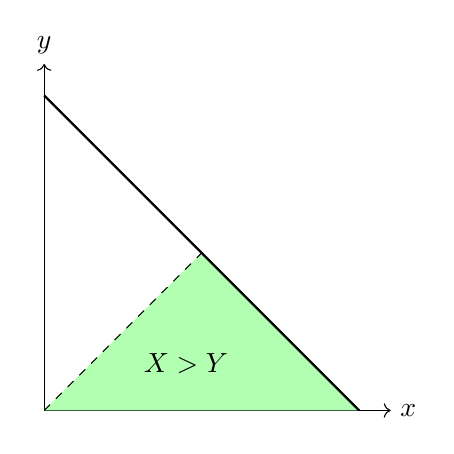
\begin{tikzpicture}[scale=4]
\draw[->] (0,0)--(1.1,0) node[right] {$x$};
\draw[->] (0,0)--(0,1.1) node[above] {$y$};
\fill[green!30] (0,0)--(1,0)--(0.5,0.5)--cycle;
\draw[thick] (1,0)--(0,1);
\draw[dashed] (0,0)--(0.5,0.5);

\node at (0.45,0.15) {$X>Y$};
		\end{tikzpicture}
\caption{Region corresponding to $X>Y$.}
\label{fig:xgreaterthany}
\end{figure}

We compute
\[\P(X>Y)=\int^{x=1}_{x=0}\int^{y=\min(x,1-x)}_{y=0} 24x(1-x-y)\,dydx.\]

Split at $x=\tfrac{1}{2}$:
\[\P(X>Y)=\ds\int^{x=1/2}_{x=0}\ds\int^{y=x}_{y=0}24x(1-x-y)\,dydx+
\ds\int^{x=1}_{x=1/2}\ds\int^{y=1-x}_{y=0}24x(1-x-y)\,dydx.\]

Evaluating both integrals gives
\[\boxed{\P(X>Y)=\frac34.}\]

%%%%%%%%%%%%%%%%%%%%%%%%%%%%%%%%%%%%%%%%%%%%%%%%%%%%%%%%%%%%%%%%%%%%%%%%%%%%%%%%%%%%%%%%%%%%%%%%%%%%%%
\subsection*{Problem 4: Compute $\mathbb P(X>\tfrac{1}{2})$}
%%%%%%%%%%%%%%%%%%%%%%%%%%%%%%%%%%%%%%%%%%%%%%%%%%%%%%%%%%%%%%%%%%%%%%%%%%%%%%%%%%%%%%%%%%%%%%%%%%%%%%

The region is $\frac12 \le x \le 1$, and $0\le y\le 1-x$. See Figure~\ref{fig:xgreaterhalf}

\begin{figure}[h!]
	\centering
		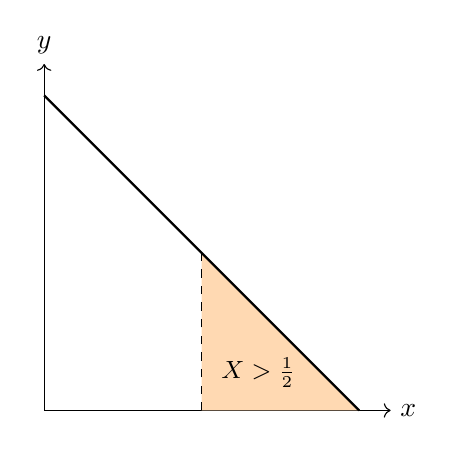
\begin{tikzpicture}[scale=4]
\draw[->] (0,0)--(1.1,0) node[right] {$x$};
\draw[->] (0,0)--(0,1.1) node[above] {$y$};
\fill[orange!30] (0.5,0)--(1,0)--(0.5,0.5)--cycle;
\draw[thick] (1,0)--(0,1);
\draw[dashed] (0.5,0)--(0.5,0.5);
\node at (0.68,0.12) {\small $X>\frac12$};
		\end{tikzpicture}
\caption{Region corresponding to $X>\tfrac12$.}
\label{fig:xgreaterhalf}
\end{figure}

Compute
\[\P\left(X>\tfrac12\right)=\int^{x=1}_{x=1/2}\int^{y=1-x}_{y=0}24x(1-x-y)\,dydx.\]
which gives us
\[\P\left(X>\tfrac12\right)=\int_{1/2}^ 12x(1-x)^2\,dx=\boxed{\frac{5}{16}.}\]


%%%%%%%%%%%%%%%%%%%%%%%%%%%%%%%%%%%%%%%%%%%%%%%%%%%%%%%%%%%%%%%%%%%%%%%%%%%%%%%%%%%%%%%%%%%%%%%%%%%%%%
\subsection*{Key Takeaways}
%%%%%%%%%%%%%%%%%%%%%%%%%%%%%%%%%%%%%%%%%%%%%%%%%%%%%%%%%%%%%%%%%%%%%%%%%%%%%%%%%%%%%%%%%%%%%%%%%%%%%%

\begin{itemize}
\item Validity of a joint density is checked by integrating over its support.
\item Joint probabilities are computed by integrating $f_{X,Y}$ over geometric regions.
\item Visualizing the support makes limits of integration immediate.
\item Different probability questions correspond to different subregions of the same support.
\end{itemize}


%%%%%%%%%%%%%%%%%%%%%%%%%%%%%%%%%%%%%%%%%%%%%%%%%%%%%%%%%%%%%%%%%%%%%%%%%%%%%%%%%%%%%%%%%%%%%%%%%%%%%%
\section*{Marginal Distributions: Interpretation, Visuals, and Examples}
%%%%%%%%%%%%%%%%%%%%%%%%%%%%%%%%%%%%%%%%%%%%%%%%%%%%%%%%%%%%%%%%%%%%%%%%%%%%%%%%%%%%%%%%%%%%%%%%%%%%%%

The joint distribution of $(X,Y)$ describes how two variables behave together.
A \emph{marginal distribution} describes the behavior of one variable alone,
ignoring the other.

%%%%%%%%%%%%%%%%%%%%%%%%%%%%%%%%%%%%%%%%%%%%%%%%%%%%%%%%%%%%%%%%%%%%%%%%%%%%%%%%%%%%%%%%%%%%%%%%%%%%%%%
\subsection*{Discrete Case:}
%%%%%%%%%%%%%%%%%%%%%%%%%%%%%%%%%%%%%%%%%%%%%%%%%%%%%%%%%%%%%%%%%%%%%%%%%%%%%%%%%%%%%%%%%%%%%%%%%%%%%%

Suppose $(X,Y)$ has a discrete joint pmf $p_{_{X,Y}}(x,y)$, displayed as a table.
Marginalization corresponds to summing highlighted cells. See Figure~\ref{discretemarginals}.

\medskip

\begin{figure}[h!]
\begin{center}
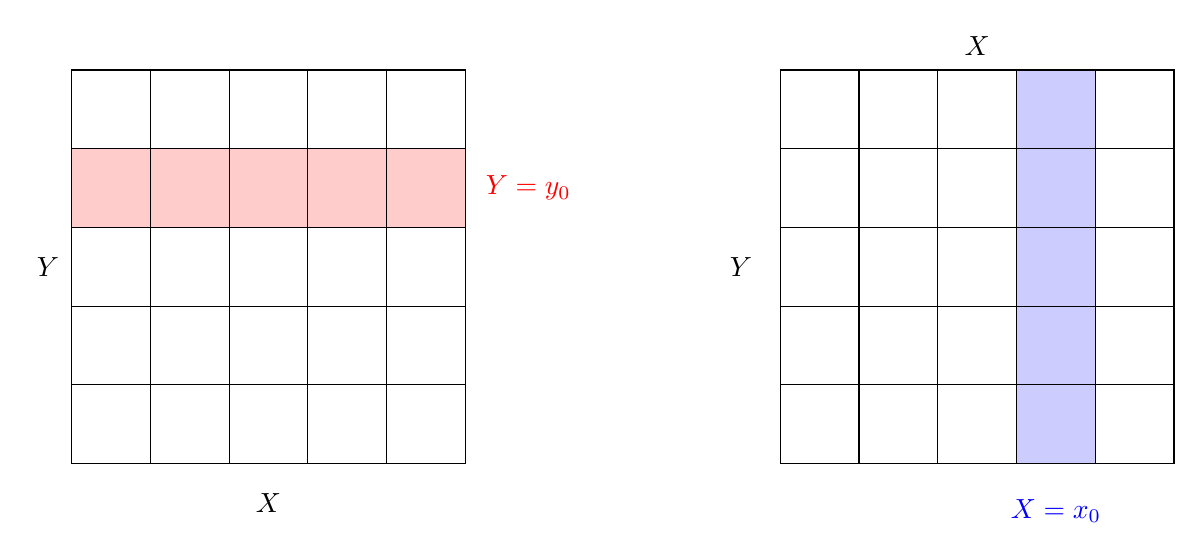
\begin{tikzpicture}[scale=1]

% ---------------- LEFT: Row sum ----------------
\begin{scope}
%\node at (2.5,5.8) {\textbf{Marginal of $Y$}};
% Shade row (row 4 now)
\fill[red!20] (0,3) rectangle (5,4);
% Grid
\draw (0,0) rectangle (5,5);
\foreach \x in {1,2,3,4} \draw (\x,0) -- (\x,5);
\foreach \y in {1,2,3,4} \draw (0,\y) -- (5,\y);
% Labels
\node at (2.5,-0.5) {$X$};
\node at (-0.3,2.5) {$Y$};
\node[red] at (5.8,3.5) {$Y=y_0$};
\end{scope}

% ---------------- RIGHT: Column sum ----------------
\begin{scope}[xshift=9cm]
%\node at (2.5,5.8) {\textbf{Marginal of $X$}};
% Shade column (column 4)
\fill[blue!20] (3,0) rectangle (4,5);
% Grid
\draw (0,0) rectangle (5,5);
\foreach \x in {1,2,3,4} \draw (\x,0) -- (\x,5);
\foreach \y in {1,2,3,4} \draw (0,\y) -- (5,\y);
% Labels
\node at (2.5,5.3) {$X$};
\node at (-0.5,2.5) {$Y$};
\node[blue] at (3.5,-0.6) {$X=x_0$};
\end{scope}
\end{tikzpicture}
\end{center}

\begin{center}
\begin{minipage}[t]{0.4\textwidth}
Fixing $Y=y_0$ and summing across the shaded row produces
\[p_{_Y}(y_0) = \sum_x p_{_{X,Y}}(x,y_0).\]
\end{minipage}
\hfill
\begin{minipage}[t]{0.4\textwidth}
Fixing $X=x_0$ and summing down the shaded column produces
\[p_{_X}(x_0) = \sum_y p_{_{X,Y}}(x_0,y).\]
\end{minipage}
\end{center}
\caption{Discrete Marginals $P_{_Y}(y)$ and $P_{_X}(x)$.}
\label{discretemarginals}
\end{figure}



\textbf{Example (Two Fair Dice).}
For two fair dice, $p_{_{X,Y}}(x,y)=1/36$ for all $x,y\in\{1,\dots,6\}$.
Summing across any row yields $p_{_X}(x)=1/6$, and summing down any column yields
$p_Y(y)=1/6$.


%%%%%%%%%%%%%%%%%%%%%%%%%%%%%%%%%%%%%%%%%%%%%%%%%%%%%%%%%%%%%%%%%%%%%%%%%%%%%%%%%%%%%%%%%%%%%%%%%%%%%%
\subsection*{Continuous Case:}
%%%%%%%%%%%%%%%%%%%%%%%%%%%%%%%%%%%%%%%%%%%%%%%%%%%%%%%%%%%%%%%%%%%%%%%%%%%%%%%%%%%%%%%%%%%%%%%%%%%%%%

Now suppose $(X,Y)$ has a joint pdf $f_{_{X,Y}}(x,y)$.
To obtain the marginal density of $X$, we integrate the joint density
along a thin vertical strip.

\medskip

\ni Fix a value $x$ and consider the strip $x \le X \le x+\delta$. This strip includes \emph{all values of $Y$} compatible with $X$ in that range. The probability of landing in the strip is approximately
\[\int f_{_{X,Y}}(x,y)\,\delta\,dy.\]

\ni Dividing by $\delta$ and letting $\delta\to 0$ yields
\[f_{_X}(x)=\int_{-\infty}^{\infty} f_{_{X,Y}}(x,y)\,dy.\]

\medskip

\begin{figure}[h!]
	\begin{center}
		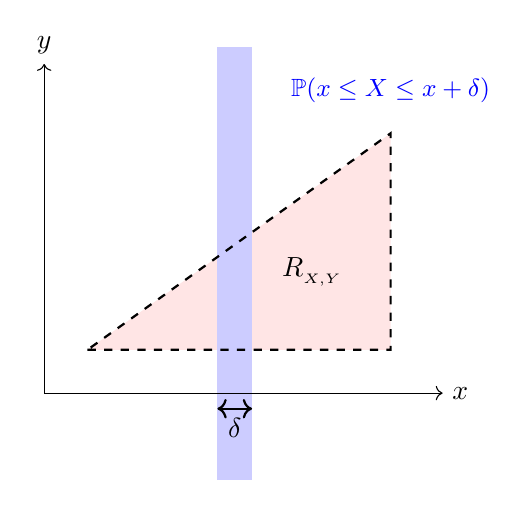
\begin{tikzpicture}[scale=1.1]
%Shaded support
\fill[red!20,opacity=0.5] (0.5,0.5) -- (4,0.5) -- (4,3) -- cycle;
% Delta strip
\fill[blue!20] (2,-1) -- (2.4,-1) -- (2.4,4) -- (2,4) -- cycle;
% Axes
\draw[->] (0,0) -- (4.6,0) node[right] {$x$};
\draw[->] (0,0) -- (0,3.8) node[above] {$y$};
% Wedge support
\draw[thick,dashed] (0.5,0.5) -- (4,0.5) -- (4,3) -- cycle;
\node at (3.1,1.4) {$R_{_{X,Y}}$};
% Delta width
\draw[thick,<->] (2,-0.18) -- (2.4,-0.18);
\node at (2.2,-0.4) {$\delta$};
\node[blue] at (4,3.5) {\small $\P(x\le X\le x+\delta)$};
		\end{tikzpicture}
	\end{center}
\caption{$\P(x < X \le x+\delta)$ over $R_{_{X,Y}} = \{(x,y) \mid 0 \le y \le x \le 1\}$}
\label{fig:contmarginal}
\end{figure}

\ni The shaded strip captures all outcomes whose $x$-coordinate lies in
$[x,x+\delta]$, regardless of $y$, but only where the joint density is nonzero.

\medskip

\textbf{Example (Triangular Support).}
Suppose $(X,Y)$ has joint pdf
\[f_{_{X,Y}}(x,y)=\left\{\begin{array}{lcl}
2&:& 0\le y\le x\le 1,\\
0&:& \text{otherwise}.
\end{array}
\right.\]

\ni The marginal density of $X$ is
\[f_{_X}(x)=\int^{y=x 2}_{y=0}\,dy=2x,\qquad 0\le x\le 1.\]

\ni Thus $X$ has an increasing density on $[0,1]$, reflecting the expanding vertical
slice of the triangular support as $x$ increases.

\medskip

In both the discrete and continuous settings, marginalization corresponds to
\emph{collapsing the joint distribution onto one axis} by summing or integrating
over the other variable.


%%%%%%%%%%%%%%%%%%%%%%%%%%%%%%%%%%%%%%%%%%%%%%%%%%%%%%%%%%%%%%%%%%%%%%%%%%%%%%%%%%%%%%%%%%%%%%%%%%%%%%
\subsection*{Example 3: Uniform Density on a Rectangle}
%%%%%%%%%%%%%%%%%%%%%%%%%%%%%%%%%%%%%%%%%%%%%%%%%%%%%%%%%%%%%%%%%%%%%%%%%%%%%%%%%%%%%%%%%%%%%%%%%%%%%%

Suppose $(X,Y)$ has joint pdf
\[f_{_{X,Y}}(x,y)=\left\{\begin{array}{lcl}
1&:& 0\le x\le 1,\; 0\le y\le 1, \\[2mm]
0&:& \text{otherwise}.
\end{array}
\right.\]

\ni The marginal density of $X$ is
\[f_{_X}(x)=\int_0^1 1\,dy = 1,\qquad 0\le x\le 1.\]

\ni Thus $X$ is uniformly distributed on $[0,1]$.
An identical calculation shows that $Y$ is also uniformly distributed on $[0,1]$.


%%%%%%%%%%%%%%%%%%%%%%%%%%%%%%%%%%%%%%%%%%%%%%%%%%%%%%%%%%%%%%%%%%%%%%%%%%%%%%%%%%%%%%%%%%%%%%%%%%%%%%
\subsection*{Example 4: Marginal Density of $Y$ when $f_{_{X,Y}}(x,y)=24x(1-x-y)$.}
%%%%%%%%%%%%%%%%%%%%%%%%%%%%%%%%%%%%%%%%%%%%%%%%%%%%%%%%%%%%%%%%%%%%%%%%%%%%%%%%%%%%%%%%%%%%%%%%%%%%%%

Returning to a previous worked example with $f_{_{X,Y}}(x,y)=24x(1-x-y)$, the marginal density of $Y$ is obtained by integrating the joint density over $x$:

\[f_{_Y}(y)=\int^{x=1-y}_{x=0}f_{_{X,Y}}(x,y)\,dx=\int^{x=1-y}_{x=0}24x(1-x-y)\,dx,\quad 0\le y \le 1.\]

\textbf{Compute the integral:}

\[\int^{x=1-y}_{x=0}24x(1-x-y)\,dx=24\int^{x=1-y}_{x=0}x - x^2 - xy\,dx
=24\left[\frac{x^2}{2}-\frac{x^3}{3}-\frac{y x^2}{2}\right]^{x=1-y}_{x=0}.\]

So the marginal density is:

\[\boxed{f_{_Y}(y)=4(1-y)^3,\quad 0 \le y \le 1.}\]

\begin{figure}[h!]
\centering
\begin{tikzpicture}[xscale=4, yscale=0.9]
\draw[->] (0,0)--(1.1,0) node[right] {$y$};
\draw[->] (0,0)--(0,4.5) node[above] {$f_{_Y}(y)$};
\draw[thick,blue] plot[domain=0:1,samples=50] (\x,{4*(1-\x)^3});
\node at (0.25,0.8) {$f_{_Y}(y)$};
\node at (-0.05,-0.2) {0};
\node at (1,-0.25) {1};
\node at (-0.05,4) {4};
\end{tikzpicture}
\caption{Marginal density $f_{_Y}(y) = 4(1-y)^3$.}
\end{figure}

%%%%%%%%%%%%%%%%%%%%%%%%%%%%%%%%%%%%%%%%%%%%%%%%%%%%%%%%%%%%%%%%%%%%%%%%%%%%%%%%%%%%%%%%%%%%%%%%%%%%%%
\subsection*{Example 5: Distribution Function $F_{_Y}(y)$ when $f_{_{X,Y}}(x,y)=24x(1-x-y)$.}
%%%%%%%%%%%%%%%%%%%%%%%%%%%%%%%%%%%%%%%%%%%%%%%%%%%%%%%%%%%%%%%%%%%%%%%%%%%%%%%%%%%%%%%%%%%%%%%%%%%%%%

The distribution function is

\[F_{_Y}(y)=\P(Y\le y)=\int^{t=y}_{t=0}f_{_Y}(t)\,dt = \int^{t=y}_{t=0}4(1-t)^3\,dt.\]

Compute:

\[\int^{t=y}_{t=0}4(1-t)^3\,dt=-(1-t)^4\Big|^{t=y}_{t=0}=-(1-y)^4+1^4=1-(1-y)^4.\]

\[\boxed{F_{_Y}(y) = 1 - (1-y)^4, \quad 0 \le y \le 1.}\]

\begin{figure}[h!]
	\centering
		\begin{tikzpicture}[scale=4]
% Axes
\draw[->] (-0.2,0)--(1.3,0) node[right] {$y$};
\draw[->] (0,0)--(0,1.1) node[above] {$F_Y(y)$};
% Extended CDF: constant 0 for y<0
\draw[thick,blue] (-0.2,0) -- (0,0);
% Main increasing part 0<=y<=1
\draw[thick,blue] plot[domain=0:1,samples=50] (\x,{1-(1-\x)^4});
% Extended CDF: constant 1 for y>1
\draw[thick,blue] (1,1) -- (1.3,1);
% Label
\node at (0.35,0.5) {$F_Y(y)$};
% Optional tick marks
\foreach \x in {0,1}
  \draw (\x,0.02) -- (\x,-0.02) node[below] {$\x$};
\foreach \y in {1}
  \draw (0.02,\y) -- (-0.02,\y) node[left] {$\y$};
		\end{tikzpicture}
\caption{Distribution function $F_{_Y}(y) = 1-(1-y)^4$, showing $F_{_Y}(y)=0$ for $y<0$ and $F_{_Y}(y)=1$ for $y>1$.}
\label{fig:distplot2}
\end{figure}



%%%%%%%%%%%%%%%%%%%%%%%%%%%%%%%%%%%%%%%%%%%%%%%%%%%%%%%%%%%%%%%%%%%%%%%%%%%%%%%%%%%%%%%%%%%%%%%%%%%%%%
\section*{Independence of Random Variables}
%%%%%%%%%%%%%%%%%%%%%%%%%%%%%%%%%%%%%%%%%%%%%%%%%%%%%%%%%%%%%%%%%%%%%%%%%%%%%%%%%%%%%%%%%%%%%%%%%%%%%%

Two random variables are called \emph{independent} if knowing the value of one provides
no information about the other.

\medskip

In practice, independence is identified through simple factorization tests.

%%%%%%%%%%%%%%%%%%%%%%%%%%%%%%%%%%%%%%%%%%%%%%%%%%%%%%%%%%%%%%%%%%%%%%%%%%%%%%%%%%%%%%%%%%%%%%%%%%%%%%
\subsection*{Discrete Case}
%%%%%%%%%%%%%%%%%%%%%%%%%%%%%%%%%%%%%%%%%%%%%%%%%%%%%%%%%%%%%%%%%%%%%%%%%%%%%%%%%%%%%%%%%%%%%%%%%%%%%%

If $(X,Y)$ is discrete, then $X$ and $Y$ are independent if and only if
\[
p_{_{X,Y}}(x,y)=p_{_X}(x)\,p_{_Y}(y)\qquad\text{for all }x,y.\]

\ni When this condition holds, the joint pmf table can be reconstructed
from its row and column sums.

\medskip

\textbf{Example (Two Fair Dice):} For two fair dice,
\[p_{_{X,Y}}(x,y)=\frac{1}{36}=\frac{1}{6}\cdot\frac{1}{6}=p_{_X}(x)p_{_Y}(y),\]
so the outcomes of the two dice are independent.

%%%%%%%%%%%%%%%%%%%%%%%%%%%%%%%%%%%%%%%%%%%%%%%%%%%%%%%%%%%%%%%%%%%%%%%%%%%%%%%%%%%%%%%%%%%%%%%%%%%%%%
\subsection*{Continuous Case}
%%%%%%%%%%%%%%%%%%%%%%%%%%%%%%%%%%%%%%%%%%%%%%%%%%%%%%%%%%%%%%%%%%%%%%%%%%%%%%%%%%%%%%%%%%%%%%%%%%%%%%

If $(X,Y)$ is continuous, then $X$ and $Y$ are independent if and only if
\[f_{_{X,Y}}(x,y)=f_{_X}(x)\,f_{_Y}(y)\qquad\text{for all }(x,y).\]

\ni In this case, the joint density separates into a product of two one-dimensional densities.

\medskip

\textbf{Example:} If $X$ and $Y$ are independent and uniformly distributed on $[0,1]$, then
\[f_{_{X,Y}}(x,y)=1,\qquad 0\le x\le 1,\;0\le y\le 1,\]
corresponding to a constant density over a rectangle.

%%%%%%%%%%%%%%%%%%%%%%%%%%%%%%%%%%%%%%%%%%%%%%%%%%%%%%%%%%%%%%%%%%%%%%%%%%%%%%%%%%%%%%%%%%%%%%%%%%%%%%
\subsection*{Geometric Interpretation}
%%%%%%%%%%%%%%%%%%%%%%%%%%%%%%%%%%%%%%%%%%%%%%%%%%%%%%%%%%%%%%%%%%%%%%%%%%%%%%%%%%%%%%%%%%%%%%%%%%%%%%

\ni Independence has a clear geometric meaning.

\begin{itemize}
\item In the discrete case, probabilities factor across rows and columns of the table.
\item In the continuous case, the joint density forms a \emph{rectangular surface}
with no interaction between $x$ and $y$.
\end{itemize}

\ni Non-rectangular supports or densities that do not factor indicate dependence.

\medskip

Independence is therefore a strong structural property of a joint distribution,
not merely a numerical coincidence.


%%%%%%%%%%%%%%%%%%%%%%%%%%%%%%%%%%%%%%%%%%%%%%%%%%%%%%%%%%%%%%%%%%%%%%%%%%%%%%%%%%%%%%%%%%%%%%%%%%%%%%
\section*{Practice Problems}
%%%%%%%%%%%%%%%%%%%%%%%%%%%%%%%%%%%%%%%%%%%%%%%%%%%%%%%%%%%%%%%%%%%%%%%%%%%%%%%%%%%%%%%%%%%%%%%%%%%%%%

The following problems are intended for in-class work and guided practice.
Some focus on foundational skills (setting up integrals, identifying support),
while others require deeper geometric or conceptual reasoning.

\bigskip

%%%%%%%%%%%%%%%%%%%%%%%%%%%%%%%%%%%%%%%%%%%%%%%%%%%%%%%%%%%%%%%%%%%%%%%%%%%%%%%%%%%%%%%%%%%%%%%%%%%%%%
\subsection*{Foundational Practice}
%%%%%%%%%%%%%%%%%%%%%%%%%%%%%%%%%%%%%%%%%%%%%%%%%%%%%%%%%%%%%%%%%%%%%%%%%%%%%%%%%%%%%%%%%%%%%%%%%%%%%%

\begin{enumerate}

\item
Let $(X,Y)$ have joint density
\[
f_{X,Y}(x,y)=
\begin{cases}
6y(1-x), & 0 \le x \le 1,\; 0 \le y \le 1,\\
0, & \text{otherwise}.
\end{cases}
\]

\begin{enumerate}
\item Verify that $f_{X,Y}$ is a valid joint density.
\item Sketch the support of $(X,Y)$.
\item Compute the marginal density $f_X(x)$.
\item Compute $\P(X \le \tfrac12)$.
\end{enumerate}

\bigskip

\item
Suppose $(X,Y)$ has joint pdf
\[
f_{X,Y}(x,y)=
\begin{cases}
2, & 0 \le y \le x \le 1,\\
0, & \text{otherwise}.
\end{cases}
\]

\begin{enumerate}
\item Compute the marginal densities $f_X(x)$ and $f_Y(y)$.
\item Find $\P(Y \le \tfrac14)$.
\item Describe in words why $f_X(x)$ is increasing on $[0,1]$.
\end{enumerate}

\bigskip

\item
Let $(X,Y)$ be discrete with joint pmf given by
\[
p_{X,Y}(x,y)=\frac{1}{10}, \qquad
(x,y)\in\{(0,0),(0,1),(1,0),(1,1),(2,0),(2,1),(3,0),(3,1),(4,0),(4,1)\}.
\]

\begin{enumerate}
\item Construct a table for the joint pmf.
\item Find the marginal pmfs $p_X(x)$ and $p_Y(y)$.
\item Are $X$ and $Y$ independent? Justify your answer.
\end{enumerate}

\end{enumerate}

\bigskip

%%%%%%%%%%%%%%%%%%%%%%%%%%%%%%%%%%%%%%%%%%%%%%%%%%%%%%%%%%%%%%%%%%%%%%%%%%%%%%%%%%%%%%%%%%%%%%%%%%%%%%
\subsection*{Challenge Problems (In-Class Discussion)}
%%%%%%%%%%%%%%%%%%%%%%%%%%%%%%%%%%%%%%%%%%%%%%%%%%%%%%%%%%%%%%%%%%%%%%%%%%%%%%%%%%%%%%%%%%%%%%%%%%%%%%

\begin{enumerate}

\item
Let $(X,Y)$ have joint density
\[
f_{X,Y}(x,y)=
\begin{cases}
c(x+y), & 0 \le x \le 1,\; 0 \le y \le 1,\\
0, & \text{otherwise}.
\end{cases}
\]

\begin{enumerate}
\item Find the constant $c$.
\item Compute $\P(X+Y \le 1)$.
\item Determine whether $X$ and $Y$ are independent.
\end{enumerate}

\bigskip

\item
Suppose $(X,Y)$ has joint pdf
\[
f_{X,Y}(x,y)=
\begin{cases}
k, & 0 \le y \le x^2 \le 1,\\
0, & \text{otherwise}.
\end{cases}
\]

\begin{enumerate}
\item Sketch the support of $(X,Y)$.
\item Find $k$.
\item Compute the marginal density $f_X(x)$.
\end{enumerate}

\bigskip

\item
Let $(X,Y)$ have joint density
\[
f_{X,Y}(x,y)=24x(1-x-y), \qquad x\ge0,\; y\ge0,\; x+y\le1.
\]

\begin{enumerate}
\item Compute $\P(Y > X)$.
\item Compute $\P(X+Y > \tfrac12)$.
\item Without computing, explain whether $\P(X>Y)$ should be greater or less than $\tfrac12$.
\end{enumerate}

\bigskip

\item
Let $F_{X,Y}(x,y)$ be a joint distribution function that is constant in $x$ for all $x>2$.

\begin{enumerate}
\item What does this imply about the support of $(X,Y)$?
\item What does it say about the marginal distribution of $Y$?
\item Give an example of a joint density with this property.
\end{enumerate}

\end{enumerate}

\bigskip

%%%%%%%%%%%%%%%%%%%%%%%%%%%%%%%%%%%%%%%%%%%%%%%%%%%%%%%%%%%%%%%%%%%%%%%%%%%%%%%%%%%%%%%%%%%%%%%%%%%%%%
\subsection*{Reflection Prompt (Optional)}
%%%%%%%%%%%%%%%%%%%%%%%%%%%%%%%%%%%%%%%%%%%%%%%%%%%%%%%%%%%%%%%%%%%%%%%%%%%%%%%%%%%%%%%%%%%%%%%%%%%%%%

\begin{quote}
Many joint distributions are defined by geometric regions in the plane.
Which aspects of these problems depended more on geometry than algebra?
How does sketching the support change the way you think about probabilities?
\end{quote}

\vfill\eject


%%%%%%%%%%%%%%%%%%%%%%%%%%%%%%%%%%%%%%%%%%%%%%%%%%%%%%%%%%%%%%%%%%%%%%%%%%%%%%%%%%%%%%%%%%%%%%%%%%%%%%
\section*{Solutions to Practice Problems}
%%%%%%%%%%%%%%%%%%%%%%%%%%%%%%%%%%%%%%%%%%%%%%%%%%%%%%%%%%%%%%%%%%%%%%%%%%%%%%%%%%%%%%%%%%%%%%%%%%%%%%

%%%%%%%%%%%%%%%%%%%%%%%%%%%%%%%%%%%%%%%%%%%%%%%%%%%%%%%%%%%%%%%%%%%%%%%%%%%%%%%%%%%%%%%%%%%%%%%%%%%%%%
\subsection*{Foundational Practice}
%%%%%%%%%%%%%%%%%%%%%%%%%%%%%%%%%%%%%%%%%%%%%%%%%%%%%%%%%%%%%%%%%%%%%%%%%%%%%%%%%%%%%%%%%%%%%%%%%%%%%%

\begin{enumerate}

\item
\textbf{Solution.}

\begin{enumerate}
\item Since $f_{X,Y}(x,y)\ge0$ and
\[
\int_0^1\int_0^1 6y(1-x)\,dy\,dx
=6\int_0^1(1-x)\,dx\int_0^1 y\,dy
=6\cdot\frac12\cdot\frac12=1,
\]
the function is a valid joint density.

\item The support is the unit square $[0,1]\times[0,1]$.

\item
\[
f_X(x)=\int_0^1 6y(1-x)\,dy
=3(1-x),\qquad 0\le x\le1.
\]

\[
\boxed{f_X(x)=3(1-x)}
\]

\item
\[
\P(X\le\tfrac12)=\int_0^{1/2}3(1-x)\,dx
=\frac{9}{8}.
\]

\[
\boxed{\P(X\le\tfrac12)=\tfrac{9}{8}}
\]
\end{enumerate}

\bigskip

\item
\textbf{Solution.}

\begin{enumerate}
\item
\[
f_X(x)=\int_0^x 2\,dy = 2x,\qquad
f_Y(y)=\int_y^1 2\,dx = 2(1-y).
\]

\[
\boxed{f_X(x)=2x,\quad f_Y(y)=2(1-y)}
\]

\item
\[
\P(Y\le\tfrac14)=\int_0^{1/4}2(1-y)\,dy=\frac{7}{16}.
\]

\[
\boxed{\P(Y\le\tfrac14)=\tfrac{7}{16}}
\]

\item The density increases with $x$ because larger values of $x$ allow a wider vertical range for $y$.
\end{enumerate}

\bigskip

\item
\textbf{Solution.}

\begin{enumerate}
\item Each allowed pair has probability $1/10$.

\item
\[
p_X(x)=\sum_y p_{X,Y}(x,y)=\frac{2}{10},\qquad
p_Y(y)=\sum_x p_{X,Y}(x,y)=\frac{5}{10}.
\]

\item Since $p_{X,Y}(x,y)\ne p_X(x)p_Y(y)$, $X$ and $Y$ are not independent.

\[
\boxed{X \text{ and } Y \text{ are not independent}}
\]
\end{enumerate}

\end{enumerate}

%%%%%%%%%%%%%%%%%%%%%%%%%%%%%%%%%%%%%%%%%%%%%%%%%%%%%%%%%%%%%%%%%%%%%%%%%%%%%%%%%%%%%%%%%%%%%%%%%%%%%%
\subsection*{Challenge Problems}
%%%%%%%%%%%%%%%%%%%%%%%%%%%%%%%%%%%%%%%%%%%%%%%%%%%%%%%%%%%%%%%%%%%%%%%%%%%%%%%%%%%%%%%%%%%%%%%%%%%%%%

\begin{enumerate}

\item
\textbf{Solution.}

\begin{enumerate}
\item
\[
1=c\int_0^1\int_0^1(x+y)\,dy\,dx
=c.
\]

\[
\boxed{c=1}
\]

\item The region $x+y\le1$ is a right triangle of area $1/2$.

\[
\P(X+Y\le1)=\int_0^1\int_0^{1-x}(x+y)\,dy\,dx=\frac13.
\]

\[
\boxed{\P(X+Y\le1)=\tfrac13}
\]

\item The density does not factor, so $X$ and $Y$ are not independent.

\[
\boxed{X \text{ and } Y \text{ are not independent}}
\]
\end{enumerate}

\bigskip

\item
\textbf{Solution.}

\begin{enumerate}
\item The support is the region below $y=x^2$ for $0\le x\le1$.

\item
\[
1=k\int_0^1 x^2\,dx=\frac{k}{3}
\quad\Rightarrow\quad k=3.
\]

\[
\boxed{k=3}
\]

\item
\[
f_X(x)=\int_0^{x^2}3\,dy=3x^2.
\]

\[
\boxed{f_X(x)=3x^2}
\]
\end{enumerate}

\bigskip

\item
\textbf{Solution.}

\begin{enumerate}
\item By symmetry,
\[
\P(Y>X)=\frac12.
\]

\[
\boxed{\P(Y>X)=\tfrac12}
\]

\item
\[
\P(X+Y>\tfrac12)=1-\int_0^{1/2}\int_0^{1/2-x}24x(1-x-y)\,dy\,dx.
\]

Evaluating,
\[
\P(X+Y>\tfrac12)=\frac{23}{24}.
\]

\[
\boxed{\P(X+Y>\tfrac12)=\tfrac{23}{24}}
\]

\item Since the density increases with $x$, $X>Y$ is slightly more likely than $Y>X$.
\end{enumerate}

\bigskip

\item
\textbf{Solution.}

\begin{enumerate}
\item The support of $X$ is contained in $(-\infty,2]$.
\item $Y$ has a proper marginal distribution.
\item Example:
\[
f_{X,Y}(x,y)=e^{-y}\mathbf{1}_{\{0\le x\le2,\; y\ge0\}}.
\]
\end{enumerate}

\end{enumerate}


%%%%%%%%%%%%%%%%%%%%%%%%%%%%%%%%%%%%%%%%%%%%%%%%%%%%%%%%%%%%%%%%%%%%%%%%%%%%%%%%%%%%%%%%%%%%%%%%%%%%%%%
%\section*{The R Code:} 
%%%%%%%%%%%%%%%%%%%%%%%%%%%%%%%%%%%%%%%%%%%%%%%%%%%%%%%%%%%%%%%%%%%%%%%%%%%%%%%%%%%%%%%%%%%%%%%%%%%%%%%
% Here is the R code used for the above simulations.
%\vspace*{2mm}
%\small 
%\begin{lstlisting}[language=R]
%
%
%
%\end{lstlisting}



\vskip 1cm
\hrule
\vskip 5mm
\begin{center}
\bf Please let me know if you have any questions, comments, or corrections!
\end{center}

%%%%%%%%%%%%%%%%%%%%%%%%%%%%%%%%%%%%%%%%%%%%%%%%%%%%%%
\end{document}
%%%%%%%%%%%%%%%%%%%%%%%%%%%%%%%%%%%%%%%%%%%%%%%%%%%%%%

